\documentclass[aspectratio=169]{beamer}

%\includeonlyframes{current}

\usepackage[utf8]{inputenc}
\usepackage[american]{babel}
\usepackage{amsmath,amsthm}
\usepackage{unicode}
\usepackage{array,tabularx}
\usepackage{ifthen}
\usepackage{tikz}
\usetikzlibrary{matrix,decorations,decorations.text,calc,arrows,snakes,shapes,positioning}
\usepackage{tikzsymbols}
\usepackage[backend=biber,citestyle=authoryear-comp,bibstyle=beamer,doi=false,isbn=false,url=true,maxnames=10]{biblatex}
\bibliography{refs}

\usepackage{ulem}

\mode<presentation>{%
  \usetheme{ibm}
}

\newcommand{\C}{ℂ}
\newcommand{\R}{ℝ}
\newcommand{\Z}{ℤ}
\newcommand{\N}{ℕ}
\newcommand{\Q}{ℚ}
\newcommand{\F}{\mathbb{F}}
\renewcommand{\P}{\mathbb{P}}
\renewcommand{\O}{\mathcal{O}}
\newcommand{\tildO}{\mathcal{\tilde{O}}}
\newcommand{\poly}{\operatorname{poly}}
\newcommand{\polylog}{\operatorname{polylog}}
\newcommand{\End}{\operatorname{End}}
\newcommand{\Hom}{\operatorname{Hom}}
\newcommand{\Gal}{\operatorname{Gal}}
\newcommand{\chr}{\operatorname{char}}
\newcommand{\Cl}{\operatorname{Cl}}
\newcommand{\GL}{\operatorname{GL}}
\renewcommand{\a}{{\mathfrak{a}}}
\renewcommand{\b}{{\mathfrak{b}}}
\newcommand{\g}{{\mathfrak{g}}}
\newcommand{\G}{{\mathcal{G}}}
\newcommand{\E}{{\mathcal{E}}}
\newcommand{\cyc}[1]{{〈 #1 〉}}
\newcommand{\ord}{\operatorname{ord}}
\newcommand{\mat}[1]{\left(\begin{smallmatrix}#1\end{smallmatrix}\right)}
\newcommand{\from}{\overset{\$}{\leftarrow}}

\newcommand{\bl}[1]{\textcolor{blue}{#1}}
\newcommand{\rd}[1]{\textcolor{red}{#1}}
\newcommand{\gr}[1]{\textcolor{green}{#1}}
\newcommand{\og}[1]{\textcolor{orange}{#1}}

\definecolor{light blue}{RGB}{0,102,204}

\newcommand{\myedge}[3]{
  \draw[#3] (360/\crater*#1 : \diam) to[bend right] (360/\crater*#2 : \diam);
}
\newcommand{\sk}[4]{
  \draw[very thick,blue]   (0,0) -- (0,#1);
  \draw[very thick,red]    (1,0) -- (1,#2);
  \draw[very thick,green]  (2,0) -- (2,#3);
  \draw[very thick,orange] (3,0) -- (3,#4);
}

\newenvironment<>{goodblock}[1]{%
  \begin{actionenv}#2%
      \def\insertblocktitle{#1}%
      \par%
      \mode<presentation>{%
        \setbeamercolor{block title}{fg=green!60!black,bg=green!50!white}
       \setbeamercolor{block body}{bg=green!20!white}
     }%
      \usebeamertemplate{block begin}}
    {\par\usebeamertemplate{block end}\end{actionenv}}
\newenvironment<>{mehblock}[1]{%
  \begin{actionenv}#2%
      \def\insertblocktitle{#1}%
      \par%
      \mode<presentation>{%
        \setbeamercolor{block title}{fg=yellow!50!black,bg=yellow!50!white}
       \setbeamercolor{block body}{bg=yellow!20!white}
     }%
      \usebeamertemplate{block begin}}
    {\par\usebeamertemplate{block end}\end{actionenv}}
\newenvironment<>{badblock}[1]{%
  \begin{actionenv}#2%
      \def\insertblocktitle{#1}%
      \par%
      \mode<presentation>{%
        \setbeamercolor{block title}{fg=red!60!black,bg=red!50!white}
       \setbeamercolor{block body}{bg=red!20!white}
     }%
      \usebeamertemplate{block begin}}
    {\par\usebeamertemplate{block end}\end{actionenv}}


../share/isographs.tex

\title[Isogeny Based Cryptography]{Isogeny Based Cryptography}
\subtitle{towards standardization and beyond}
\author{Luca De Feo}
\date[Nov 6, 2020~~~~ICSP 2020]{November 6, 2020\\
  ICSP 2020}
\institute{IBM Research Zürich}

\begin{document}

\frame[plain]{\titlepage}

%%

\begin{frame}{Why isogenies?}
  \begin{columns}
    \begin{column}{0.45\textwidth}
      Six families still in NIST post-quantum competition:
      
      \bigskip
      \begin{tabular}{ >{\color{structure}}l@{\hspace{2em}} c c}
        Lattices     & 5 encryption & \textcolor{black!30}{2 signature} \\
        Codes        & 3 encryption\\
        Multivariate & & \textcolor{black!30}{2 signature}\\
        Isogenies    & \alert{1 encryption}\\
        Hash-based   & & \textcolor{black!30}{1 signature}\\
        MPC          & & \textcolor{black!30}{1 signature}
      \end{tabular}
    \end{column}
    \begin{column}{0.45\textwidth}<2->
      \centering
      \begin{overlayarea}{0.8\textwidth}{\textheight}
        \begin{onlyenv}<2>
          \begin{tikzpicture}
            \node at (3,-0.5) {\bf Public key size};
            \node at (3,-1) {NIST-1 level (AES128)};
            \node at (3,-1.5) {\footnotesize (not to scale)};
            \draw (0.5,0) -- (5.5,0);
            \fill[structure] (1,0) -- (2,0) -- (2,4) -- (1,4);
            \node at (1.5,4.5) {\parbox{2cm}{\centering \emph{Codes}\\1 -- 300 KB}};
            \fill[structure] (2.5,0) -- (3.5,0) -- (3.5,1) -- (2.5,1);
            \node at (3,1.8) {\parbox{2cm}{\centering \emph{Lattices}\\0.5 -- 10 KB}};
            \fill[structure] (4,0) -- (5,0) -- (5,0.2) -- (4,0.2);
            \node at (4.5,0.7) {\parbox{2cm}{\centering \emph{Isogenies}\\209 B}};
          \end{tikzpicture}
        \end{onlyenv}
        \transdissolve<3>
        \begin{onlyenv}<3->
          \begin{tikzpicture}
            \node at (3,-0.5) {\bf Encryption performance};
            \node at (3,-1) {NIST-1 level (AES128)};
            \node at (3,-1.5) {\footnotesize (not to scale)};
            \draw (0.5,0) -- (5.5,0);
            \fill[structure] (1,0) -- (2,0) -- (2,0.2) -- (1,0.2);
            \node at (1.5,0.7) {\parbox{2cm}{\centering \emph{Codes}\\1 Mcycles}};
            \fill[structure] (2.5,0) -- (3.5,0) -- (3.5,0.3) -- (2.5,0.3);
            \node at (3,1) {\parbox{2cm}{\centering \emph{Lattices}\\0.5 -- 5 Mcycles}};
            \fill[structure] (4,0) -- (5,0) -- (5,4) -- (4,4);
            \node at (4.5,4.5) {\parbox{2cm}{\centering \emph{Isogenies}\\190 Mcycles}};
          \end{tikzpicture}
        \end{onlyenv}
      \end{overlayarea}
    \end{column}
  \end{columns}
\end{frame}

%%

\begin{frame}

  \vfill
  
  \begin{quotation}
    ``We found that CECPQ2 ([NTRU] the ostrich) outperformed CECPQ2b
    ([SIKE] the turkey), for the majority of connections in the
    experiment, indicating that \textbf{fast algorithms with large
      keys may be more suitable for TLS than slow algorithms with
      small keys}. However, \textbf{we observed the opposite}---that
    CECPQ2b outperformed CECPQ2---\textbf{for the slowest connections
      on some devices}, including Windows computers and Android mobile
    devices. One possible explanation for this is packet fragmentation
    and packet loss.''
  \end{quotation}

  \begin{flushright}
    --- K. Kwiatkowski, L. Valenta (Cloudflare)\\
    \emph{The TLS Post-Quantum Experiment}\\
    \small \url{https://blog.cloudflare.com/the-tls-post-quantum-experiment/}
  \end{flushright}
\end{frame}

%% 

\begin{frame}{Elliptic curves}
  \begin{columns}
    \begin{column}{0.4\textwidth}
      Elliptic curves:
      
      \[y^2 = x^3 + ax + b\]
      
      Define a \emph{group law} such that any three colinear points
      add up to zero.

      \begin{itemize}
      \item The law is \emph{algebraic}\\ (it has \textit{formulas});
      \item The law is \emph{commutative};
      \item $\O$ is the \emph{group identity};
      \end{itemize}
    \end{column}
    \begin{column}{0.6\textwidth}
      \begin{center}
        \begin{tikzpicture}[domain=-2.4566:4,samples=100,yscale=1/2]
          \draw plot (\x,{sqrt(\x*\x*\x-4*\x+5)});
          \draw plot (\x,{-sqrt(\x*\x*\x-4*\x+5)});

          \draw[thin,gray,-latex] (0,-7) -- (0,7);
          \draw[thin,gray,-latex] (-3,0) -- (4,0);
          \draw (-3,1) -- (4,8/3+3);
          \begin{scope}[every node/.style={draw,circle,inner sep=1pt,fill},cm={1,2/3,0,0,(0,3)}]
            \node at (-2.287980,0) {};
            \node at (-0.535051,0) {};
            \node at (3.267475,0) {};
          \end{scope}
          \begin{scope}[every node/.style={yshift=0.3cm},cm={1,2/3,0,0,(0,3)}]
            \node at (-2.287980,0) {$P$};
            \node at (-0.535051,0) {$Q$};
            \node at (3.267475,0) {$R$};
          \end{scope}

          \draw[dashed] (3.267475,3.267475*2/3+3) -- (3.267475,-3.267475*2/3-3) 
          node[draw,circle,inner sep=1pt,fill] {}
          node[xshift=-0.1cm,anchor=east] {$P+Q$};
        \end{tikzpicture}
      \end{center}
    \end{column}
  \end{columns}
\end{frame}

%%

\begin{frame}
  \frametitle{Maps: what's \alt<2->{\xout{scalar multiplication} an
      isogeny}{scalar multiplication}?}

  \begin{overlayarea}{\textwidth}{4em}
    \Large
    \[
      \alt<3->{\phi}{[n]}
      \;:\; P \mapsto
      \alt<3->{\phi(P)}{\underbrace{P + P + \cdots + P}_{n\text{ times}}}\]
  \end{overlayarea}
  
  \begin{itemize}
  \item A map \emph{$E\to \alt<4->{\xout{E} E'}{E\phantom{\xout{}}}$},
  \item a \emph{group morphism},
  \item with \emph{finite kernel}\\
    \alt<5->{(\xout{the torsion group $E[n]\simeq(ℤ/nℤ)^2$} any
      finite subgroup \emph{$H\subset E$})}{(the torsion group
      \emph{$E[n]\simeq(ℤ/nℤ)^2$})},
  \item \emph{surjective} (in the algebraic closure),
  \item given by \emph{rational maps} of degree \alt<6->{\xout{$n^2$}
      \emph{$\#H$}}{\emph{$n^2$}}.
  \end{itemize}

  \medskip
  
  \begin{uncoverenv}<7->
    (Separable) isogenies $\Leftrightarrow$ finite subgroups:
    \alert{\[0 \to H \to E \overset{\phi}{\to} E' \to 0\]}
  \end{uncoverenv}
\end{frame}

%% 

\begin{frame}{Isogenies: an example over $\F_{11}$}
  \centering
  \begin{tikzpicture}[scale=0.4]
    \begin{scope}
      \node[anchor=center] at (0,7) {$E \;:\; y^2 = x^3 + x$};

      \uncover<-1>{
        \draw[thin,gray] (0,-6) -- (0,6);
        \draw[thin,gray] (-6,0) -- (6,0);
      }

      \foreach \x/\y in {0/0,5/3,-4/3,-3/5,-2/1,-1/3} {
        \draw[blue,fill] (\x,\y) circle (0.2) node(E_\x_\y){}
        (\x,-\y) circle (0.2) node(E_\x_-\y){};
      }

      \uncover<2->{\draw[red,fill] (0,0) circle (0.3);}
    \end{scope}

    \draw[black!10!white,thick] (10,-7) -- +(0,14);
    
    \begin{scope}[shift={(20,0)}]
      \node at (0,7) {$E' \;:\; y^2 = x^3 - 4x$};

      \uncover<-1>{
        \draw[thin,gray] (0,-6) -- (0,6);
        \draw[thin,gray] (-6,0) -- (6,0);
      }

      \foreach \x/\y in {0/0,2/0,3/2,4/2,6/4,-2/0,-1/5} {
        \draw[color=blue,fill] (\x,\y) circle (0.2) node(F_\x_\y){}
        (\x,-\y) circle (0.2) node(F_\x_-\y){};
      }
    \end{scope}

    \begin{scope}[color=red,-latex,dashed]
      \begin{uncoverenv}<2->
        \path
        (E_5_3) edge (F_3_2)
        (E_-4_3) edge (F_4_-2)
        (E_-3_5) edge (F_4_2)
        (E_-2_1) edge (F_3_-2)
        (E_-1_3) edge (F_-2_0);
      \end{uncoverenv}
      \begin{uncoverenv}<2->
        \path
        (E_5_-3) edge (F_3_-2)
        (E_-4_-3) edge (F_4_2)
        (E_-3_-5) edge (F_4_-2)
        (E_-2_-1) edge (F_3_2)
        (E_-1_-3) edge (F_-2_0);
      \end{uncoverenv}
    \end{scope}
  \end{tikzpicture}
  
  \begin{columns}
    \begin{column}{0.5\textwidth}
      \[\phi(x,y) = \left(\frac{x^2 + 1}{x},\quad y\frac{x^2-1}{x^2}\right)\]
    \end{column}
    \begin{column}{0.5\textwidth}
      \begin{itemize}
      \item<2-> Kernel generator in \alert{red}.
      \item<2-> This is a degree $2$ map.
      \item<2-> Analogous to $x\mapsto x^2$ in $\F_q^*$.
      \end{itemize}
    \end{column}
  \end{columns}
\end{frame}

%%

\begin{frame}{Up to \emph{isomorphism}}
  \begin{center}
    \begin{tikzpicture}[domain=-2.4566:4,samples=100]
      \newcount\zoomout
      \transduration<15-21>{0.5}
      \animatevalue<15-20>{\zoomout}{0}{10}
      \begin{uncoverenv}<-20>
        \begin{scope}[scale=1-0.09*\zoomout]
          \begin{scope}
            \draw[thin,gray,-latex] (0,-4) -- (0,4);
            \draw[thin,gray,-latex] (-4.2,0) -- (7,0);
          \end{scope}
          
          \newcount\xstretch
          \newcount\ystretch
          \newcount\slant
          \transduration<1-13>{0.5}
          \animatevalue<1-5>{\xstretch}{0}{4}
          \animatevalue<5-9>{\ystretch}{0}{4}
          \animatevalue<9-13>{\slant}{0}{4}      
          \begin{scope}[yscale=0.55-0.05*\the\ystretch,xscale=1+0.1*\the\xstretch,xslant=0.02*\slant]
            \draw plot (\x,{sqrt(\x*\x*\x-4*\x+5)});
            \draw plot (\x,{-sqrt(\x*\x*\x-4*\x+5)});

            \begin{uncoverenv}<-18>
              \draw (-3,1) -- (4,8/3+3);
              \begin{scope}[every node/.style={draw,circle,inner sep=1pt,fill},cm={1,2/3,0,0,(0,3)}]
                \node at (-2.287980,0) {};
                \node at (-0.535051,0) {};
                \node at (3.267475,0) {};
              \end{scope}
              \begin{scope}[every node/.style={yshift=0.3cm},cm={1,2/3,0,0,(0,3)}]
                \node at (-2.287980,0) {$P$};
                \node at (-0.535051,0) {$Q$};
                \node at (3.267475,0) {$R$};
              \end{scope}
              \draw[dashed] (3.267475,3.267475*2/3+3) -- (3.267475,-3.267475*2/3-3) 
              node[draw,circle,inner sep=1pt,fill] {}
              node[xshift=-0.1cm,anchor=east] {$P+Q$};
            \end{uncoverenv}
          \end{scope}

          \begin{uncoverenv}<14>
            \node[anchor=west] at (-4,-3) {\Large\alert{$y^2=x^3+ax+b \quad\longrightarrow\quad j\equiv 1728\frac{4a^3}{4a^3+27b^2}$}};
          \end{uncoverenv}
        \end{scope}
      \end{uncoverenv}
      
      \begin{uncoverenv}<21->
        \draw[fill] (0,0) circle (2pt) node[anchor=north] {$j=1728$};
        \uncover<22>{
          \draw (0.1,0) edge[bend left,->] node[auto] {$\phi$} (7,0);
        }
        \uncover<22->{
          \draw[fill] (7.1,0) circle (2pt) node[anchor=north] {$j=287496$};
        }
        \uncover<23->{
          \draw (0.1,0) edge[bend left,<->,red,very thick] (7,0);
        }
      \end{uncoverenv}
    \end{tikzpicture}
  \end{center}  
\end{frame}

%%

\begin{frame}{The beauty and the beast {\quad\footnotesize(credit: Lorenz Panny)}}
  \begin{overlayarea}{\textwidth}{\textheight}
    \smallskip
    \begin{center}

      \only<-2>{
        Components of particular isogeny graphs look like this:
      }
      \only<3->{
        At this time, there are \underline{\smash{two distinct families}} of systems:
      }
      \par\vspace{1ex}

      \begin{minipage}{.49\textwidth}\centering
        \begin{tikzpicture}[scale=.6,>=stealth,shorten >=.2mm,shorten <=.2mm,rotate=90,line width=.6pt]
          \isoggraph
        \end{tikzpicture}

        \vspace{.2ex}

        \only<3->{
          $\F_p$ \\[.7ex]
          \textbf{CSIDH}
          \,\raisebox{.2ex}{\small{[pron.: sea-side]}}
          \\ {\small
            \url{https://csidh.isogeny.org}
            \par}
        }
      \end{minipage}
      % 
      \begin{minipage}{.49\textwidth}\centering
        \begin{tikzpicture}[scale=2.456,>=stealth,shorten >=.2mm,shorten <=.2mm,rotate=90,line width=.6pt]
          \fpsqgraph
        \end{tikzpicture}

        \vspace{.2ex}

        \only<3->{
          $\F_{p^2}$ \\[.7ex]
          \textbf{SIDH}
          \\ {\small
            \url{https://sike.org}
            \par}
        }
      \end{minipage}

      \only<-2>{
        \vspace{3ex}

        \textit{Which of these is good for crypto?}
        \pause
        \onslide<2>{%
          \,\textbf{Both.}
        }
      }

    \end{center}
  \end{overlayarea}
\end{frame}

%%

\begin{frame}{Brief history of isogeny-based cryptography}
  \begin{description}
  \item[1997] Couveignes introduces the \emph{Hard Homogeneous Spaces}
    framework. His work stays unpublished for 10 years.
  \item[2006] Rostovtsev \& Stolbunov independently rediscover
    Couveignes ideas, suggest isogeny-based Diffie--Hellman as a
    \emph{quantum-resistant} primitive.
  \item[2006-2010] Other isogeny-based protocols by Teske and Charles,
    Goren \& Lauter.
  \item[2011-2012] D., Jao \& Plût introduce \emph{SIDH}, an
    efficient post-quantum key exchange inspired by Couveignes,
    Rostovtsev, Stolbunov, Charles, Goren, Lauter.
  \item[2017] SIDH is submitted to the NIST competition (with the name
    \emph{SIKE}, only isogeny-based candidate).
  \item[2018] Castryck, Lange, Martindale, Panny \& Renes create an
    efficient variant of the Couveignes--Rostovtsev--Stolbunov
    protocol, named \emph{CSIDH}.
  \item[2019] Isogeny signature craze: \emph{SeaSign}
    (D. \& Galbraith; Decru, Panny \& Vercauteren), \emph{CSI-FiSh}
    (Beullens, Kleinjung \& Vercauteren), \emph{VDF} (D., Masson,
    Petit \& Sanso).
  \item[2020] Isogeny signatures get interesting: \emph{SQISign}
    (D., Kohel, Leroux, Petit, Wesolowski).\\
    SIKE is an \emph{Alternate candidate finalist} in NIST's 3rd round.
  \end{description}
\end{frame}

%%

\begin{frame}{Elliptic curves}

  Let \emph{$E \;:\; y^2 = x^3 + ax + b$} be an elliptic curve\dots

  \begin{center}
    \begin{tikzpicture}[domain=-2.4566:4,samples=100]
      \newcount\rotate
      \animate<2-6>
      \animatevalue<2-6>{\rotate}{0}{90}
      \begin{scope}[rotate=-\the\rotate]
        \draw plot (\x,{0.5*sqrt(\x*\x*\x-4*\x+5)});
        \draw plot (\x,{-0.5*sqrt(\x*\x*\x-4*\x+5)});
      \end{scope}
      
      \begin{uncoverenv}<1>
        \begin{scope}[yscale=1/2]
          \draw[thin,gray,-latex] (0,-7) -- (0,7);
          \draw[thin,gray,-latex] (-3,0) -- (4,0);
          
          \draw (-3,1) -- (4,8/3+3);
          \begin{scope}[every node/.style={draw,circle,inner sep=1pt,fill},cm={1,2/3,0,0,(0,3)}]
            \node at (-2.287980,0) {};
            \node at (-0.535051,0) {};
            \node at (3.267475,0) {};
          \end{scope}
          \begin{scope}[every node/.style={yshift=0.3cm},cm={1,2/3,0,0,(0,3)}]
            \node at (-2.287980,0) {$P$};
            \node at (-0.535051,0) {$Q$};
            \node at (3.267475,0) {$R$};
          \end{scope}
          \draw[dashed] (3.267475,3.267475*2/3+3) -- (3.267475,-3.267475*2/3-3) 
          node[draw,circle,inner sep=1pt,fill] {}
          node[xshift=-0.1cm,anchor=east] {$P+Q$};
        \end{scope}
      \end{uncoverenv}
    \end{tikzpicture}
  \end{center}
\end{frame}

%%

\begin{frame}{Elliptic curves}
  \transdissolve
  \centering
  
\includegraphics[height=0.7\textheight]{ec-happy}
\end{frame}

%%

\begin{frame}{The QUANTHOM Menace}
  \centering
  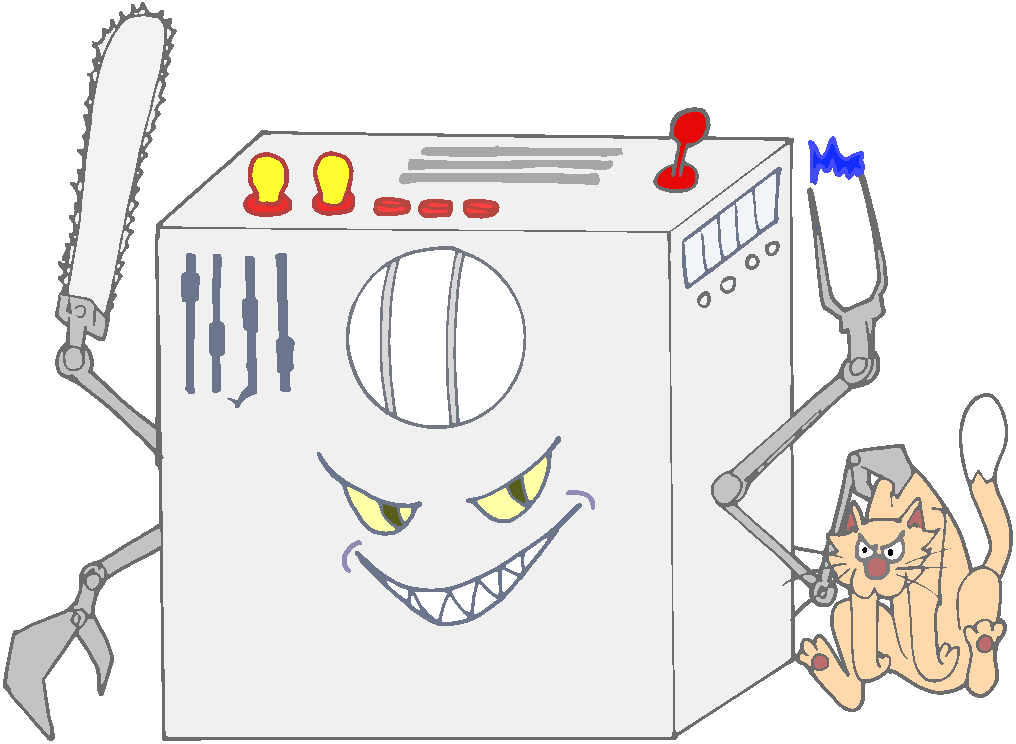
\includegraphics[height=0.7\textheight]{qc-color}
\end{frame}

%%

\begin{frame}{Basically every isogeny-based key-exchange...}
  \centering
  \begin{tikzpicture}
    \comicneue\itshape
    \node at (0,0) {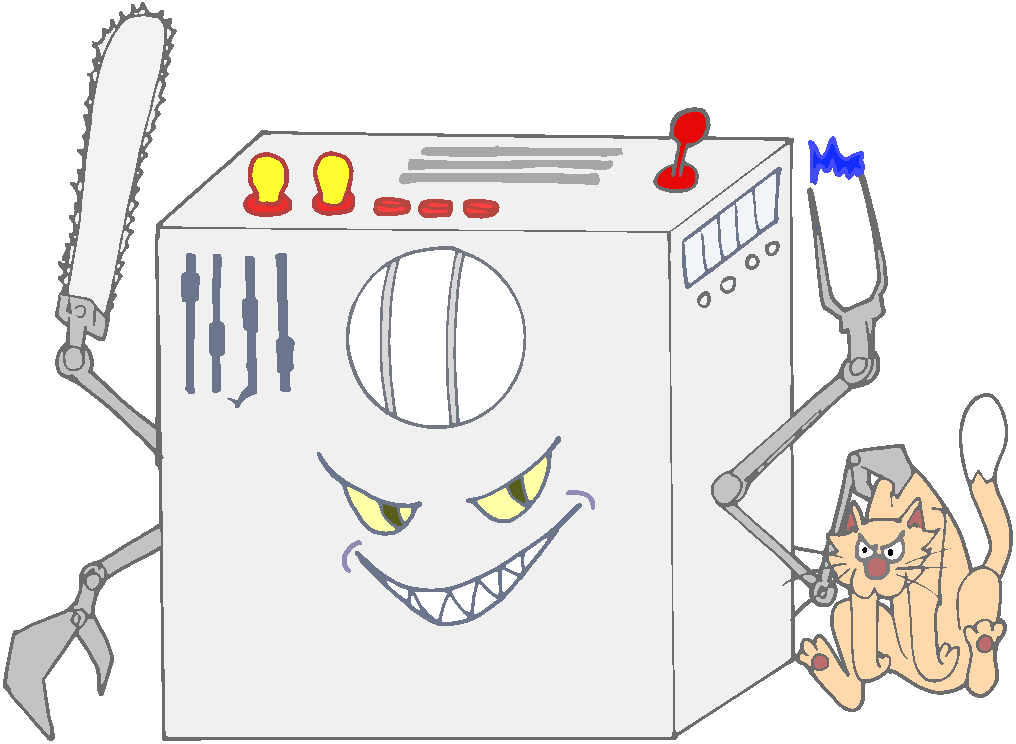
\includegraphics[height=2.5cm]{qc-color}};
    
    \node(E0) at (-6,0) {
\includegraphics[height=1cm]{ec-happy}};

    \uncover<2->{
      \node(EA) at (0,3) {
\includegraphics[height=1cm]{ec-happy}};
      \node(EB) at (0,-3) {
\includegraphics[height=1cm]{ec-happy}};
      \draw[->,decorate,decoration=snake] (E0) to (EA);
      \draw[->,decorate,decoration=snake] (E0) to (EB);
      \node[right=0.3cm of EA] {\bl{Public curve}};
      \node[right=0.3cm of EB] {\bl{Public curve}};
    }
    \uncover<3>{
      \node(ES) at (6,0) {
\includegraphics[height=1cm]{ec-happy}};
      \draw[->,decorate,decoration=snake] (EA) to (ES);
      \draw[->,decorate,decoration=snake] (EB) to (ES);
      \node[below=1em of ES] {\rd{Shared secret}};
    }
  \end{tikzpicture}
\end{frame}

%%

\begin{frame}{From 10 minutes to 10ms in 20 years}
  \begin{tikzpicture}[xscale=1.3,gray,every node/.style={anchor=south}]
    \draw[->] (0,0) -- (11,0);
    \uncover<1->{
      \node at (1,-0.5) {1997};
      \draw (1,-0.1) -- +(0,0.3) node[blue]{Couveignes' key exchange};
    }
    \uncover<2->{
      \node at (3,-0.5) {2006};
      \draw (3,-0.1) -- +(0,1.3) node[blue]{Rostovstev \& Stolbunov (> 5 min)};
    }
    \uncover<3->{
      \node at (4,-0.5) {2011};
      \draw (4,-0.1) -- +(0,2.3) node[red]{SIDH (500ms) \tiny(Jao and D.)};
    }
    \uncover<4->{
      \node at (5,-0.5) {2012};
      \draw (5,-0.1) -- +(0,3.3) node[red]{SIDH (50ms) \tiny(D., Jao, Plût)};
    }
    \uncover<5->{
      \node at (6,-0.5) {2016};
      \draw (6,-0.1) -- +(0,4.3) node[red]{SIDH (30ms) \tiny(Costello, Longa, Naherig)};
    }
    \uncover<6->{
      \node at (7,-0.5) {2017};
      \draw (7,-0.1) -- +(0,5.3) node[red]{SIKE (10ms) \tiny(NIST candidate)};
    }
    \uncover<7->{
      \node at (8,-0.5) {2018};
      \draw (8,-0.1) -- +(0,2.3) node[blue]{CSIDH (50ms)};
    }
    \uncover<8>{
      \node at (9,-0.5) {2019};
      \draw (9,-0.1) -- +(0,3.3) node[blue]{CSIDH (35ms) \tiny(Meyer, Reith)};
    }
  \end{tikzpicture}
\end{frame}

%%

\begin{frame}{CSIDH vs SIDH}
  \centering
  \vspace{-3mm}
  \begin{tabular}{l *{2}{| @{\hspace{1em}}c@{\hspace{1em}}} }
    & \textbf{CSIDH} & \textbf{SIDH}\\
    \hline
    Speed (on x64 arch., NIST 1) & $\sim$ 35ms & $\sim$ 6ms\\
    Public key size (NIST 1) & 64B & 346B\\
    Key compression & \\
    \enskip{}\rotatebox[origin=c]{180}{$\Lsh$} speed & & $\sim$ 11ms\\
    \enskip{}\rotatebox[origin=c]{180}{$\Lsh$} size & & 209B\\
    Submitted to NIST & no & yes\\
    TRL & 4 & 6\\
    \hline
    Best classical attack & $p^{1/4}$ & $p^{1/4}\;\;$ ($p^{3/8}$)\\
    Best quantum attack & $\tildO\left(3^{\sqrt{\log_3 p}}\right)$ & $p^{1/6}\;\;$ ($p^{3/8}$)\\
    Key size scales & quadratically & linearly\\
    CPA security & yes & yes\\
    CCA security & yes & Fujisaki-Okamoto\\
    Constant time & it's complicated & yes\\
    \hline
    Non-interactive key exchange & yes & no\\
    Signatures & short but (slow $\mid$ do not scale) & big and slow
  \end{tabular}
\end{frame}

%%

\begin{frame}{Proving knowledge of a secret isogeny}
  \begin{description}
  \item[Public:] Curves \emph{$E, E'$}
  \item[Secret:] An isogeny walk \emph{$E\to E'$}
  \end{description}

  \begin{block}{Why?}
    \begin{itemize}
    \item For interactive identification;
    \item For digital signatures;
    \item For validating public keys (esp. SIDH);
    \item More\dots
    \end{itemize}
  \end{block}

  \begin{block}{Some properties}
    \newcolumntype{C}{>{\centering\arraybackslash}X}
    \begin{tabularx}{\columnwidth}{l *{4}C}
      & \multicolumn{2}{c}{\small Zero knowledge}\\
      & \small Statistical & \small Computational & \small Quantum resistance & \small Usable\\
      \hline
      CSIDH & \checkmark & & \checkmark/{\footnotesize sort of} & \Xey/\Neutrey\\
      SIDH & & \checkmark & \checkmark & \Neutrey\\
      SQISign & & \checkmark & \checkmark & \Cooley\\
    \end{tabularx}
  \end{block}
\end{frame}

%%

\begin{frame}{Security assumptions in Isogeny-based Cryptography}
  \begin{goodblock}{Isogeny walk problem}
    \begin{description}
    \item[Input] Two isogenous elliptic curves \emph{$E,E'$} over
      \emph{$\F_q$}.
    \item[Output] A path \emph{$E\to E'$} in an isogeny graph.
    \end{description}
  \end{goodblock}

  \begin{mehblock}{SIDH problem (1)}
    \begin{description}
    \item[Input]
      Elliptic curves \emph{$E,E'$} over \emph{$\F_q$},
      isogenous of degree \bl{$\ell_A^{e_A}$}.
    \item[Output] The unique path \emph{$E\to E'$} of length
      \bl{$e_A$} in the \bl{$\ell_A$}-isogeny graph.
    \end{description}    
  \end{mehblock}
  
  \begin{badblock}{SIDH problem (2)}
    \begin{description}
    \item[Input]
      \begin{itemize}
      \item Elliptic curves \emph{$E,E'$} over \emph{$\F_q$},
        isogenous of degree \bl{$\ell_A^{e_A}$};
      \item The action of the isogeny on $E[\rd{\ell_B^{e_B}}]$.
      \end{itemize}
    \item[Output] The unique path \emph{$E\to E'$} of length
      \bl{$e_A$} in the \bl{$\ell_A$}-isogeny graph.
    \end{description}    
  \end{badblock}
\end{frame}

%%

\begin{frame}{A $\Sigma$-protocol from Diffie--Hellman\footnote{Kids, do
      not try this at home! Use Schnorr!}}
  \begin{columns}
    \begin{column}{0.55\textwidth}
      \begin{itemize}
      \item<1-> A key pair \emph{$(s, g^s)$};
      \item<2-> Commit to a \emph{random element $g^r$};
      \item<3-> Challenge with bit \emph{$b\in\{0,1\}$};
      \item<4-> Respond with \emph{$c = \alert<6->{r - b\cdot s\mod\#G}$};
      \item<5-> Verify that \emph{$g^c(g^s)^b = g^r$}.
      \end{itemize}

      \begin{block}{Zero-knowledge}<6->
        \centering
        Does not leak because:\\
        \alert{$c$ is uniformly distributed} and independent from $s$.
      \end{block}

      \begin{uncoverenv}<7->
        Unlike Schnorr, compatible with\\
        \emph{group action Diffie--Hellman}.
      \end{uncoverenv}
    \end{column}  
    \begin{column}{0.40\textwidth}
      \centering
      \begin{tikzpicture}
        \node (g) at (0,0) {\alt<-6>{$g$}{$E_1$}};
        \node (gs) at (3,0) {\alt<-6>{$g^s$}{$E_s$}};
        \path[->] (g) edge node[auto]{\alt<-6>{$s$}{$g^s$}} (gs);
        \uncover<2->{
          \node (gr) at (1.5,-3) {\alt<-6>{$g^r$}{$E_r$}};
          \path[->] (g) edge node[auto,swap]{\alt<-6>{$r$}{$g^r$}} (gr);
        }
        \uncover<4->{
          \path[dashed,->] (gs) edge node[auto]{\alt<-6>{$r-s$}{$g^{r-s}$}} (gr);
        }
      \end{tikzpicture}
    \end{column}  
  \end{columns}
\end{frame}

%%

\begin{frame}{The trouble with groups of unknown structure}
  \begin{columns}
    \begin{column}{0.5\textwidth}
      In CSIDH secrets look like:
      $g^{\vec{s}} = \bl{g_2^{s_2}}\rd{g_3^{s_3}}\gr{g_5^{s_5}}\cdots$
      \begin{itemize}
      \item the elements $g_i$ are fixed,
      \item the secret is the exponent vector
        \emph{$\vec{s}=(s_2,s_3,\dots)\in[-B,B]^n$},
      \item secrets must be sampled in a box \emph{$[-B,B]^n$} ``large
        enough''\dots
      \end{itemize}

      \begin{block}{The leakage}<2->%
        With \emph{$\vec{s},\vec{r}\from[-B,B]^n$}, the distribution of
        \emph{$\vec{r}-\vec{s}$} \alert{depends on the long term secret $\vec{s}$!}
      \end{block}
    \end{column}
    \begin{column}{0.45\textwidth}
      \centering
      \begin{tikzpicture}[scale=0.3]
        \draw (-2,2) node{$+B$} (-2,-2) node{$-B$};
        \draw (0,0) -- (18,0);
        \draw[dotted] (0,2) -- (18,2) (0,-2) -- (18,-2);

        \draw (8,-4) node {\Large$-$};
        
        \draw (-2,-6) node{$+B$} (-2,-10) node{$-B$};
        \draw (0,-8) -- (18,-8);
        \draw[dotted] (0,-6) -- (18,-6) (0,-10) -- (18,-10);

        \uncover<2->{
          \draw (8,-12) node {\Large$=$};
        
          \draw (-2,-15) node{$+B$} (-2,-19) node{$-B$};
          \draw (0,-17) -- (18,-17);
          \draw[dotted] (0,-15) -- (18,-15) (0,-19) -- (18,-19);
        }
      
        \foreach \i in {0,...,18} {
          \pgfmathparse{round(2.2*sin(140*\i))}
          \let\s\pgfmathresult
          \pgfmathparse{round(2.2*cos(125*\i))}
          \let\r\pgfmathresult
          \draw[very thick] (\i,0) -- (\i,\r);
          \draw[very thick] (\i,-8) -- (\i,-8+\s);
          \uncover<2->{
            \draw[very thick] (\i,-17) -- (\i,-17+\r-\s);
          }
        }
      \end{tikzpicture}
    \end{column}
  \end{columns}
\end{frame}

%%

\begin{frame}{The two fixes}
  \begin{block}{Compute the group structure and stop whining}
    \emph{CSI-FiSh}: Beullens, Kleinjung and Vercauteren 2019
    \begin{itemize}
    \item Already suggested by Couveignes (1996) and Stolbunov (2006).
    \item Computationally intensive (\emph{subexponential parameter generation}).
    \item Decent parameters, e.g.: \emph{263 bytes, 390 ms, @NIST-1.} 
    \item[--] Technically not post-quantum (signing requires solving ApproxCVP).
   \end{itemize}
  \end{block}

  \begin{block}{Do like the lattice people}
    \emph{SeaSign}: D. and Galbraith 2019
    \begin{itemize}
    \item Use \emph{Fiat--Shamir with aborts} (Lyubashevsky 2009).
    \item[--] Huge increase in signature size and time.
    \item Compromise signature size/time with public key size (still
      slow).
    \end{itemize}
  \end{block}
\end{frame}

%%

\begin{frame}{SeaSign Performance (NIST-1)}
  \centering
  \begin{tabular}{l  c  c  c }
    & \bf $t=1$ bit challenges
    & \bf $t=16$ bits challenges
    & \bf PK compression \\
    \hline
    Sig size
    & \alert{20 KiB} & \gr{978 B} & 3136 B\\
    PK size
    & 64 B & \alert{4 MiB} & 32 B\\
    SK size
    & 32 B & 16 B & \alert{1 MiB} \\
    Est. keygen time
    & 30 ms & \alert{30 mins} & \alert{30 mins} \\
    Est. sign time
    & \alert{30 hours} & 6 mins & 6 mins \\
    Est. verify time
    & \alert{10 hours} & 2 mins & 2 mins \\
    \hline
    Asymptotic sig size
    & $O(\lambda^2\log(\lambda))$ & $O(\lambda t\log(\lambda))$ & $O(\lambda^2 t)$\\[2em]
    \multicolumn{4}{c}{\bf Speed/size compromises by Decru, Panny and Vercauteren 2019}\\
    \hline
    {Sig size}
    & 36 KiB & 2 KiB & ---\\
    {Est. sign time}
    & 30 mins & 80 s & ---\\
    {Est. verify time}
    & 20 mins & 20 s & ---
  \end{tabular}
\end{frame}

%%

\begin{frame}{CSI-FiSh~\footcite{beullens:2019}}
  \begin{itemize}
  \item Record breaking class group computation for CSIDH-512, hard to
    scale to larger primes;
  \item Effectively (but not asymptotically) makes CSIDH into an HHS:
    \begin{itemize}
    \item Compatible with secret sharing in the exponent, yields decent
      threshold signatures.\footcite{cryptoeprint:2019:1288}
    \end{itemize}
  \end{itemize}
  
  \centering
  \begin{tabular}{r r r | r r r | r r r }
    $S$ & $t$ & $k$ & $|\mathrm{sk}|$ & $|\mathrm{sk}|$ & $|\mathrm{sig}|$ & KeyGen & Sign & Verify \\
    \hline
    $2^1$    & $56$ & $16$ & 16 B & 128 B & 1880 B & 100 ms & 2.92 s & 2.92 s\\
    $2^2$    & $38$ & $14$ & 16 B & 256 B & 1286 B & 200 ms & 1.98 s & 1.97 s\\
    $2^3$    & $28$ & $16$ & 16 B & 512 B &  956 B & 400 ms & 1.48 s & 1.48 s\\
    $2^4$    & $23$ & $13$ & 16 B &  1 KB &  791 B & 810 ms & 1.20 s & 1.19 s\\
    $2^6$    & $16$ & $16$ & 16 B &  4 KB &  560 B & 3.3 s  & 862 ms & 859 ms\\
    $2^8$    & $13$ & $11$ & 16 B & 16 KB &  461 B & 13 s   & 671 ms & 670 ms\\
    $2^{10}$ & $11$ &  $7$ & 16 B & 64 KB &  395 B & 52 s   & 569 ms & 567 ms\\
    $2^{12}$ &  $9$ & $11$ & 16 B &256 KB &  329 B & 3.5 m  & 471 ms & 469 ms\\
    $2^{15}$ &  $7$ & $16$ & 16 B &  2 MB &  263 B & 28 m   & 395 ms & 393 ms
  \end{tabular}
\end{frame}

%%

\begin{frame}{A $Σ$-protocol for SIDH}
  \begin{columns}
    \begin{column}{0.6\textwidth}
      \begin{tikzpicture}
        \large
        \node[matrix of nodes, ampersand replacement=\&, column sep=3cm, row sep=1.3cm] (diagram) {
          |(E)| $E$ \& |(Es)| $E/〈\bl{S}〉$ \\
          |(Ep)| {\uncover<2->{$E/〈\rd{P}〉$}} \& |(Eps)| {\uncover<2->{$E/〈\rd{P,\bl{S}}〉$}}\\
        };
        \path[blue] (E) edge node[auto] {$\phi$} (Es);
        \uncover<2->{\path[blue] (Ep) edge node[auto,swap] {\alt<5>{$\phi'$}{\phantom{$\phi'$}?}} (Eps);}
        \uncover<2->{\path[red] (E) edge node[auto,swap] {\alt<3,6>{$\psi$}{?}} (Ep);}
        \uncover<2->{\path[red] (Eps) edge node[auto,swap] {\alt<4,6>{$\psi'$}{?}} (Es);}
      \end{tikzpicture}
    \end{column}
    \begin{column}{0.35\textwidth}
      \begin{mehblock}{$\frac{1}{3}$-soundness}
        Secret \bl{$\phi$} of degree \bl{$\ell_A^{e_A}$}.
      \end{mehblock}
    \end{column}
  \end{columns}

  \begin{enumerate}
  \item<2-> Choose a random point \rd{$P\in E[\ell_B^{e_B}]$}, compute the diagram;
  \item<2-> Publish the curves $E/〈\rd{P}〉$ and $E/〈\rd{P,\bl{S}}〉$;
  \item<3-> The verifier challenges to reveal \emph{one out of the 3}
    sides
    \begin{itemize}
    \item<3-> Isogenies \rd{$\psi,\psi'$} (degree \rd{$\ell_B^{e_B}$})
      unrelated to secret;
    \item<5-> Isogeny \bl{$\phi'$} conjectured to not reveal useful
      information on \bl{$\phi$}.
    \end{itemize}
  \end{enumerate}

  \begin{badblock}{Improving to $\frac{1}{2}$-soundness}<6->
    \begin{itemize}
    \item Reveal \rd{$\psi,\psi'$} simultaneously;
    \item Reveals action of \bl{$\phi$} on $E[\rd{\ell_B^{e_B}}]\quad⇒\quad$
      Stronger security assumption.
    \end{itemize}
  \end{badblock}
\end{frame}

%%

\begin{frame}{SIDH signature performance (NIST-1)}
  According to Yoo, Azarderakhsh, Jalali, Jao and Vladimir Soukharev
  2017:
  \begin{description}
  \item[Size:] $\approx 100 KB$,
  \item[Time:] seconds.
  \end{description}

  \pause
  
  \begin{goodblock}{Galbraith, Petit and Silva 2017}
    \begin{itemize}
    \item Concept similar to \emph{CSI-FiSh}: exploits \emph{known
        structure of endomorphism ring};
    \item Statistical zero knowledge (under heuristic assumptions);
    \item Based on the generic isogeny walk problem\\
      (requires \emph{special starting curve}, though);
    \item Size/performance comparable to Yoo \textit{et al.} (and possibly
      slower).
    \end{itemize}
  \end{goodblock}
\end{frame}

%%

\begin{frame}{SQISign: \textbf{S}hort \textbf{Q}uaternion \textbf{I}sogeny \textbf{Sign}ature}
  Signature from \emph{one round}, \emph{high soundness}
  identification protocol based on \alert{new assumption!}
    
  \emph{Most compact PQ signature scheme}: PK + Signature combined
  \textbf{5$\times$smaller} than Falcon.

  \begin{table}[h]
    \centering
    \begin{tabular}{ c c c c}
      Secret Key (bytes) & Public Key (bytes) & Signature (bytes) & Security \\
      \hline
      16 & 64 & 204 & NIST-1 \\
      \hline
    \end{tabular}
    \label{tab: key sizes}
  \end{table}

  \emph{Efficient} verification and \alert{reasonably efficient} signature.
  
  \begin{table}[h]
    \centering
    \begin{tabular}{l r r r r}
      & & Keygen & Sign & Verify \\
      \hline
      & 1st quartile & 1,922 & 7,687 & 140\\
      Mcycles & mean & 1,959 & 7,767 & 142\\
      & 3rd quartile & 2,000 & 7,909 & 148\\
      \hline
      & 1st quartile & 564 & 2,256 & 41\\
      ms & mean & 575 & 2,279 & 42\\
      & 3rd quartile & 587 & 2,321 & 43\\
      \hline
    \end{tabular}
    \label{tab:perf}
  \end{table}

  See \url{https://ia.cr/2020/1240}, or wait for Asiacrypt\dots
\end{frame}

%%

\begin{frame}{Conclusion}
  \begin{itemize}
  \item Repeat with me: \emph{I need isogeny-based crypto!}
  \item \emph{Different} isogeny graphs enable different applications,
    different \emph{security assumptions}.
  \item SIKE is \emph{here to stay}, start experimenting with it!
  \item CSIDH has \emph{still some way to go} before we gain
    confidence in it, but is going to be extremely useful in
    post-quantum applications.
  \item Post-quantum isogeny signatures are a joyous mess!
    \emph{Practically useful} isogeny signatures do exists (CSI-FiSh,
    SQISign), but a lot more research is needed to bring them to
    real-world usage.
  \end{itemize}
\end{frame}

%% 

\begin{frame}[plain]
  \centering
  \begin{tikzpicture}[remember picture,overlay]
    \begin{scope}[xscale=1.7,yshift=-15,opacity=0.8]
      \def\crater{12}
      \def\jumpa{-8}
      \def\jumpb{9}
      \def\diam{5cm}

      \foreach \i in {1,...,\crater} {
        \draw[blue] (360/\crater*\i : \diam) to[bend right] (360/\crater*\i+360/\crater : \diam);
        \draw[red] (360/\crater*\i : \diam) to[bend right] (360/\crater*\i+\jumpa*360/\crater : \diam);
        \draw[green] (360/\crater*\i : \diam) to[bend right=50] (360/\crater*\i+\jumpb*360/\crater : \diam);
      }
    \end{scope}
    
    \draw (0,0.5) node{\Huge\bf Thank you};
    \draw (0,-1.1) node{\large\url{https://defeo.lu/}};
    \draw (0,-1.8) node{\large
\includegraphics[height=0.9em]{twitter.png}~\href{https://twitter.com/luca_defeo}{@luca\_defeo}};
  \end{tikzpicture}
\end{frame}

%%

\end{document}


% LocalWords:  Isogeny abelian isogenies hyperelliptic supersingular Frobenius
% LocalWords:  isogenous
